\section{Symplectic integration.}
% Generalize your ODE program for integrating and plotting the equations of motion using the symplectic leapfrog integrator. I did not have
% time to discuss this algorithm in class today, but I’m attaching a brief
% introduction as an appendix to get you started. I will discuss this at the
% beginning of class next Thursday.
% (a) As a test, use this integrate the pendulum equations of motion in
% all regimes:
% i. rotation,
% ii. libration,
% iii. near the unstable equilibrium
A symplectic integrator is an integrator that conserve phase-space volume and Poincar\' e invariants \cite{BinneyT_}

Leapfrog integrator is a second order method that integrates ordinary differential equations. It updates the position and velocity at interleaved times. The algorithm is being implemented is of the sequence drift-kick-drift. A drift is when the position $\Vec{q}$ changes but not the momentum $\Vec{p}$ and a kick is the inverse, momentum changes but not the position. The algorithm is
\begin{align*}
    \Vec{q}_{1/2}&=\Vec{q}_0+\frac{1}{2}h\Vec{p_0}\\
    \Vec{p}&=\Vec{p}_0 + h F(\Vec{q}_{1/2})\\
    \Vec{q}&=\Vec{q}_0 + \frac{1}{2}h\Vec{p}
\end{align*}
where $F(\Vec{q}_{1/2})$

We can test the leapfrog algorithm using the pendulum. 
The equation of motion of the pendulum is given by
\begin{equation}
    \Ddot{\theta}=-\sin\theta.
\end{equation}

We can determine 3 scenarios:
\begin{itemize}
    \item Rotation \\
    It is when the total energy given by
    \begin{equation}
    E=\frac{1}{2}\Dot{\theta}^2+\left(1+\cos\theta\right)
    \end{equation}
    is bigger than the critical energy. The critical energy is given by the energy evaluated in equilibrium. For this case, is 2. If thinking of a physical pendulum, we can make the pendulum go to rotation when we start it with an added velocity.
    \item Libration \\
    It is when the total energy is smaller than the critical energy. This is where the pendulum oscillates with small amplitudes. We can achieve this when we drop the pendulum at an angle close to equilibrium.
    \item Equilibrium \\
    It is where the pendulum stays in equilibrium. This can happen when the pendulum is straight down or straight up. When it is straight up it is called an unstable equilibrium since a very small force can take it out of that state. 
\end{itemize}
This 3 scenarios can be created by using the initial conditions listed in table \ref{tab:PendulumIV}.

\begin{table}[]
    \centering
\begin{tabular}{lrr}
\toprule
{} &  $\theta$ &  $\dot{\theta}$ \\
\midrule
Rotation    &     -4.08 &             1.30 \\
Libration   &      0.50 &             0.00 \\
Near Uns Eq &      3.13 &             0.00 \\
\bottomrule
\end{tabular}

    \caption{Initial conditions use for the integration of the pendulum for the case of rotation, libration and near the unstable equilibrium.}
    \label{tab:PendulumIV}
\end{table}

% \begin{figure}
%     \centering
%     \includegraphics{CodeAndFigures/PendulumXYPlot.pdf}
%     \caption{Plot showing the movement of the pendulum for each scenario.}
%     \label{fig:pendulumOrbitPlot}
% \end{figure}

% Figure \ref{fig:pendulumOrbitPlot} shows the trajectory of the pendulum for each scenario. 

\begin{figure*}[ht!]
    \centering
    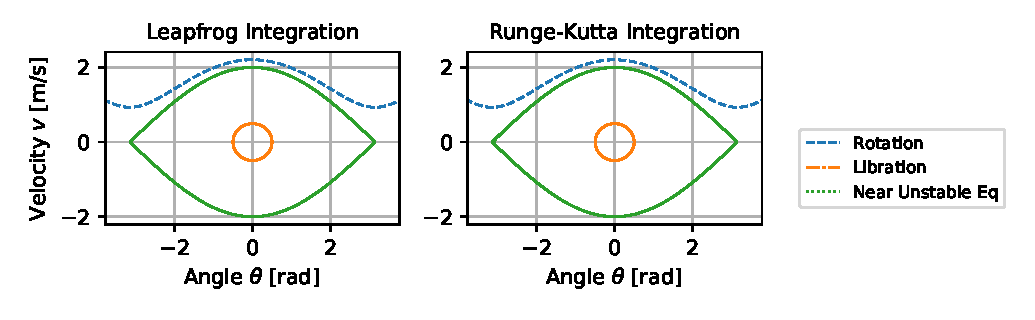
\includegraphics{CodeAndFigures/PendulumPhaseSpace.pdf}
    \caption{Plot of the phase space for each scenario using Leapfrog and 4th order Runge-Kutta (RK4).}
    \label{fig:pendulumPhaseSpace}
\end{figure*}

Figure \ref{fig:pendulumPhaseSpace} shows the phase space of each scenario using leapfrog integration and 4th order Runge-Kutta. When the pendulum is in libration it forms concentric circles near the stable equilibrium while in rotation it forms curve lines above the critical energy. When the pendulum is near the unstable equilibrium it forms an oblate shape where it almost touches the unstable equilibrium point. 
% (b) Demonstrate that the leapfrog integrator is second-order accurate
% in the sense that errors in $\mathbf{q}$ and $\mathbf{p}$ after a time step $h$ are $O(h^3)$.

\begin{figure*}[ht!]
    \centering
    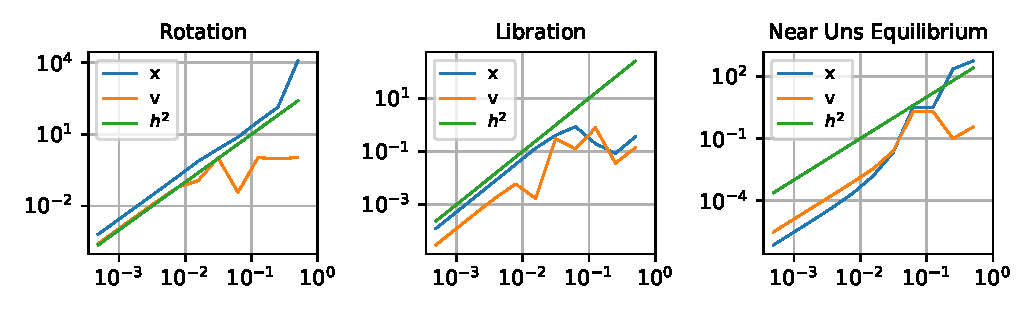
\includegraphics[width=\textwidth]{CodeAndFigures/PendulumErrorvsStepsize.pdf}
    \caption{Plots of errors at different time steps $h$ for each scenario: rotation, libration and near unstable equilibrium.}
    \label{fig:pendulumErrors}
\end{figure*}

Figure \ref{fig:pendulumErrors} shows the errors in position and velocity of leapfrog with different time steps. The error was calculated by subtracting the final value of position at a time step minus the final value at the previous time step, where the time step at each iteration gets halved. 

Note that at smaller time steps the error $\mathcal{O}(h^3)$ ie. the error is of second order represented by the line $h^2$. At larger time steps, equivalently the time steps is almost the same as the orbit period so it will suffer from variation equivalent to under sampling a signal in digital systems.

% (c) Compute the energy conservation for the trajectories in each regime
% over about 10,000 orbital periods. Compare the energy conservation for RK4 and leapfrog.
\begin{figure*}[ht!]
    \centering
    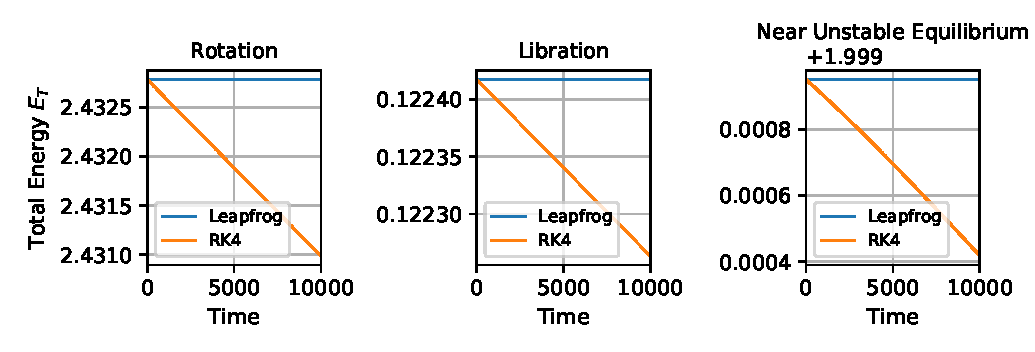
\includegraphics{CodeAndFigures/PendulumRK4vsLeapfrog.pdf}
    \caption{Plots comparing the calculated total energy through time using leapfrog integrator and RK4 integrator for each scenario of the pendulum system.}
    \label{fig:pendulumEnergy}
\end{figure*}

Figure \ref{fig:pendulumEnergy} shows the total energy of the pendulum of the 3 scenarios over 10,000 orbits. It shows that when using the leapfrog integrator, the energy has small variations but remains constant in a small range through time, in other words, energy is being conserved, while the total energy using RK4 shows a drift, energy is not conserved. This is one of the advantages of leapfrog over RK4 for dynamical systems where the energy needs to be conserved.

\clearpage